% Conversion LaTeX du fichier Word "1-AnalyseFonctionnelle2022(1).docx"
% Images extraites dans le dossier ./images
% Fichier prévu pour être inclus dans votre projet kaobook / cours existant.
% Packages nécessaires dans le préambule principal : graphicx, xcolor, hyperref, longtable, booktabs, array, calc, multirow, ulem.

\graphicspath{{images/}}
\providecommand{\ul}[1]{\uline{#1}}

\setchapterimage{../../Style/FondPoly.png}
\setchapterpreamble[u]{\margintoc}

\begingroup
\definecolor{kaoblue}{RGB}{0,82,155}
\addtokomafont{chapter}{\color{kaoblue}}
\chapter*{Introduction à l'ingénierie système}
\endgroup
\setcounter{chapter}{1}


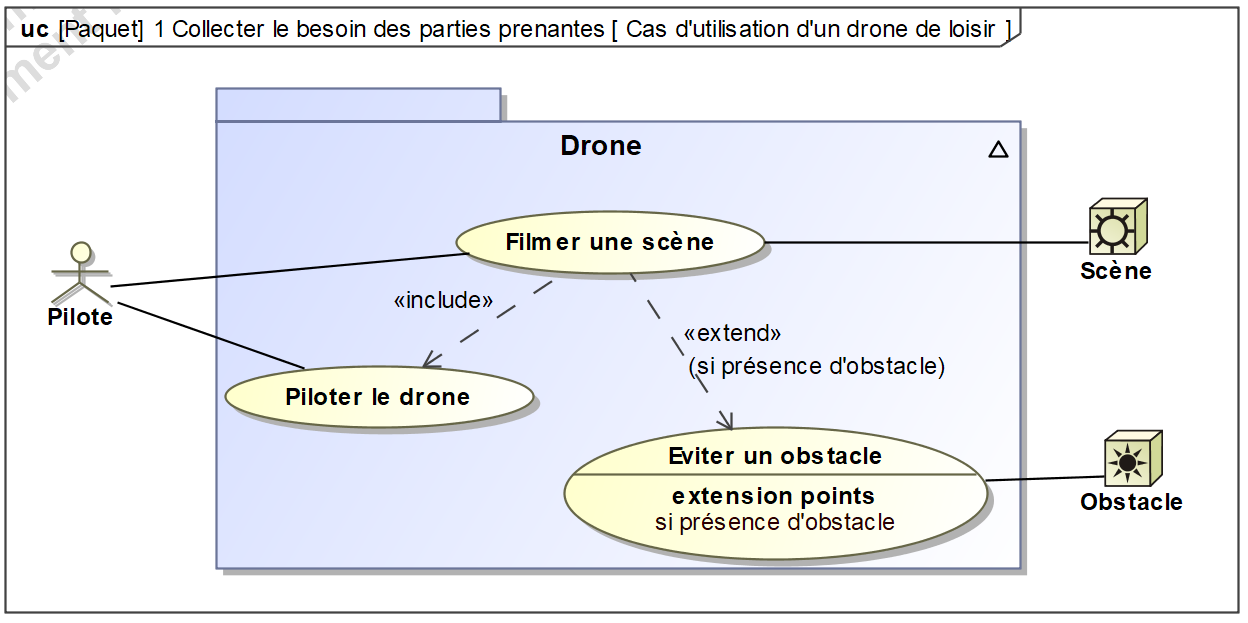
\includegraphics[width=\linewidth]{images/image3.png}

%\tableofcontents
\clearpage

\input{01_AnalyseFonctionnelle2022_contenu}
